\subsection*{Overview}
As the Food-101 dataset mostly consisted of meals \textcite{food101}, I decided to extend the
dataset slightly be including some single foods such as:
\begin{itemize}
    \item{cheese}
    \item{grapes}
    \item{banana}
    \item{apple}
    \item{orange}
    \item{spaghetti}
    \item{roll}
\end{itemize}

In order to collect these images, I used the ImageNet repository to search for
these foods individually and then downloaded the subset of images to be included
with Food 101 \textcite{imagenet}. I ran the retrain.py script on the extended dataset as in
Experiment 5.

\subsection*{Network Architecture}
The Inception V3 Model was used for this experiment.

\subsection*{Dataset}
In this experiment I extended the Food-101 dataset.

\subsection*{Libraries}
Tensorflow and numpy are used in the retrain.py script.

\subsection*{Script}
As seen in Experiment 5.

\subsection*{Results}
For this model, I achieved an accuracy of 55.3\%.

For example, an image of a banana, see \ref{fig:banana} was fed into the model with
the followng results:
\begin{itemize}
    \item{banana 0.9962}
    \item{orange 0.0009}
    \item{cheese 0.0003}
    \item{frozen yoghurt carpaccio 0.0002}
    \item{churros 0.0001}
\end{itemize}
 
\begin{figure}
    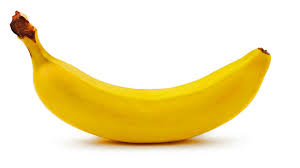
\includegraphics{banana}
    \caption{Banana}
    \label{fig:banana}
\end{figure}

\subsection*{Analysis}
The slight increase in accuracy in Experiment 5, from 54.8\% to 55.3\%, makes
sense. Since the model was pre-trained using the ImageNet dataset and all the
new images I used were from ImageNet, we would expect a higher classification
accuracy on the new additions to the dataset. This would overall increase the
average classification accuracy.
